%%%%%%
%%%%%%%%%%%%%%%%%%%%%%%%%%%%%% Title Page Info %%%%%%%%%%%%%%%%%%%%%%%%%%%%%%%%%%%%%%%%%%%
%%%%%%%%%%%%%%%%%%%%%%%%%%%%%%%%%%%%%%%%%%%%%%%%%%%%%%%%%%%%%%%%%%%%%%%%%%%%%%%%%%%%%%%%%%

\documentclass[aspectratio=169,compress]{beamer}
\mode<presentation> 

\usetheme{Warsaw}
%\usecolortheme[rgb={0.0,0.5,1.0}]{structure}
\usecolortheme[rgb={1.0,0.5,0.0}]{structure}
%\usecolortheme[rgb={0,0.4,0}]{structure}
%\usetheme{AnnArbor}

% define
\usepackage{beamerouterthememiniframes} % Para los puntitos  
\setbeamertemplate{footline}[frame number]{}

% include packages
\usepackage{subfigure}
\usepackage{multicol}
\usepackage{amsmath}
\usepackage{epsfig}
\usepackage{graphicx}
\usepackage[all,knot]{xy}
\usepackage{algorithmic}
\xyoption{arc}
\usepackage{url}
\usepackage{multimedia}
\usepackage{hyperref}
\usepackage{soul} % Resaltado de texton

\usepackage{pgfpages}
\setbeameroption{hide notes} % Only slides
%\setbeameroption{show only notes} % Only notes
%\setbeameroption{show notes on second screen=right} % Both

%\title{Recopilación del Estado del Arte de los Sistemas Inteligentes de Monitoreo Ambiental en Tamaulipas}
\title{Oportunidades de Monitoreo Ambiental Inteligente en Tamaulipas}

\author{Dr. Marco Aurelio Nu\~no-Maganda}
\institute{Universidad Politécnica de Victoria\\ Laboratorio de Sistemas Inteligentes \\
mnunom@upv.edu.mx  \vspace{.25cm} }

\date{Agosto 2022}
%\textbf{nmaganda@ccc.inaoep.mx}

%%%%%%%%%%%%%%%%%%%%%%%%%%%%%%%%%%%%%%%%%%%%%%%%%%%%%%%%%%%%%%%%%%%%%%%%%%%%%%%%%%%%%%%%%%
%%%%%%%%%%%%%%%%%%%%%%%%%%%%%% Begin Your Document %%%%%%%%%%%%%%%%%%%%%%%%%%%%%%%%%%%%%%%
%%%%%%%%%%%%%%%%%%%%%%%%%%%%%%%%%%%%%%%%%%%%%%%%%%%%%%%%%%%%%%%%%%%%%%%%%%%%%%%%%%%%%%%%%%

 

%\usepackage[backend=biber,maxcitenames=50,maxbibnames=50,sorting=ydmdddnt]{biblatex}
\usepackage[backend=biber,maxcitenames=50,maxbibnames=50,sorting=none]{biblatex}

\DeclareSortingScheme{ydmdddnt}{ 
  \sort{ 
    \field{presort} 
  } 
  \sort[final]{ 
    \field{sortkey} 
  } 
  \sort[direction=descending]{ 
    \field{year} 
  } 
  \sort[direction=descending]{ 
    \field{month} 
  } 
  \sort[direction=descending]{ 
    \field{day} 
  } 
  \sort{ 
    \field{journaltitle} 
  } 
  \sort{ 
    \field{author} 
    \field{editor} 
  } 
  \sort{ 
    \field{title} 
  } 
}




%\renewrobustcmd{\mkbibfootnote}{\normalsize\footnotemark\footnotetext}
\setbeamerfont{footnote}{size=\tiny}

\setbeamertemplate{footline}[frame number]{} % Evita que \pause 
\setbeamertemplate{bibliography item}{\insertbiblabel} % Numeros en las referenicas en vez de iconos







\newcommand{\ArchivoPrincipal}{Todos}
\newcommand{\ArchivoSecundario}{Bibliografia}


%Append keywords to identify different bibliography entries.
\DeclareSourcemap{
  \maps[datatype=bibtex, overwrite]{
    \map{
      \perdatasource{\ArchivoPrincipal.bib}
      \step[fieldset=KEYWORDS, fieldvalue=primary, append]
    }
    \map{
      \perdatasource{\ArchivoSecundario.bib}
      \step[fieldset=KEYWORDS, fieldvalue=secundary, append]
    }    
  }
}


\addbibresource{\ArchivoPrincipal.bib}
\addbibresource{\ArchivoSecundario.bib}

\usepackage{listings}
 
 \AtBeginSection[]
{
    \begin{frame}
        \frametitle{Contenido}
        \tableofcontents[currentsection]
    \end{frame}
}

\makeatletter
\def\@makefnmark{}
\makeatletter
\setbeamertemplate{footnote}{%
  \parindent 1em\noindent
  \raggedright
  *  
  \insertfootnotetext\par
}



\begin{document}

\frame{
	%\titlepage 
	\begin{titlepage}
	\end{titlepage}
	
}

%\frame{
%\frametitle{Recopilación del Estado del Arte de los Sistemas Inteligentes de Monitoreo Ambiental en Tamaulipas}
%\begin{center}
% Fila1
%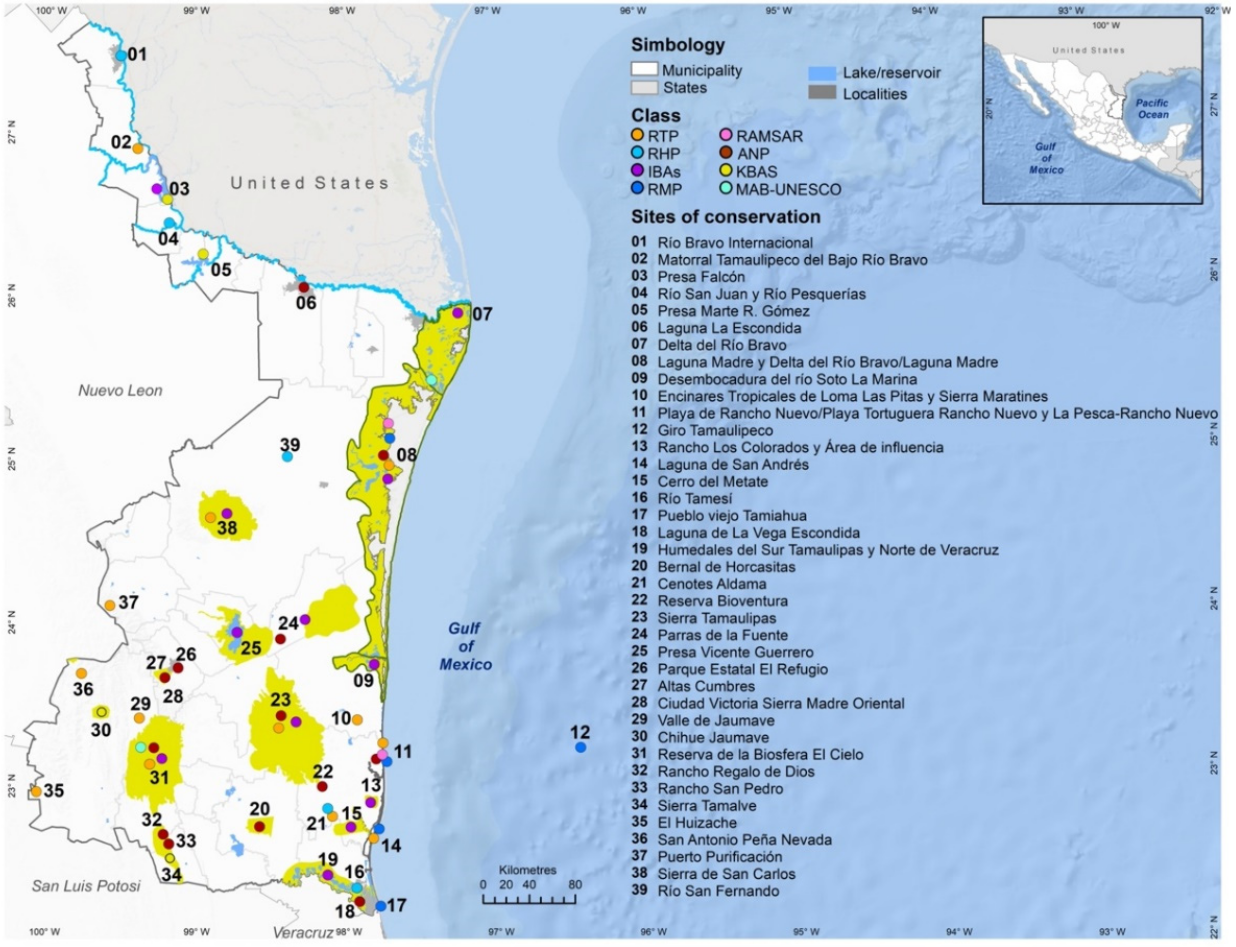
\includegraphics[width=0.50\linewidth]{figs/MapaTamps.png}\\
%\end{center}
%}

%Sitios de Conservación se clasifican en 8 tipos:
\frame{
	\frametitle{Contenido}
	\tableofcontents
}



\section[APT]{Areas protegidas de Tamaulipas}
\begin{frame}{Areas protegidas de Tamaulipas}
39 sitios importantes de conservación (Caballero-Rico et al \cite{u14010494}$^*$)
\begin{columns}
\begin{column}{0.60\textwidth}
	\begin{enumerate}  %del cuerpo académico Acuicultura Sustentable (UTMTB-CA-1)
\item Areas Protegidas
\item Regiones Terrestres Prioritarias
\item Regiones Marinas Prioritarias
\item Regiones Hidrológicas Prioritarias
\item Áreas Importantes de Aves 
\item Áreas Clave de Biodiversidad
\item Convención Relativa a los humedales de Importancia Internacional (RAMSAR)
\item UNESCO-MABs (Man and the Biosphere (MAB))
	\end{enumerate}
\end{column}

\begin{column}{0.40\textwidth}  
\begin{center}
     \begin{tabular}{cc}
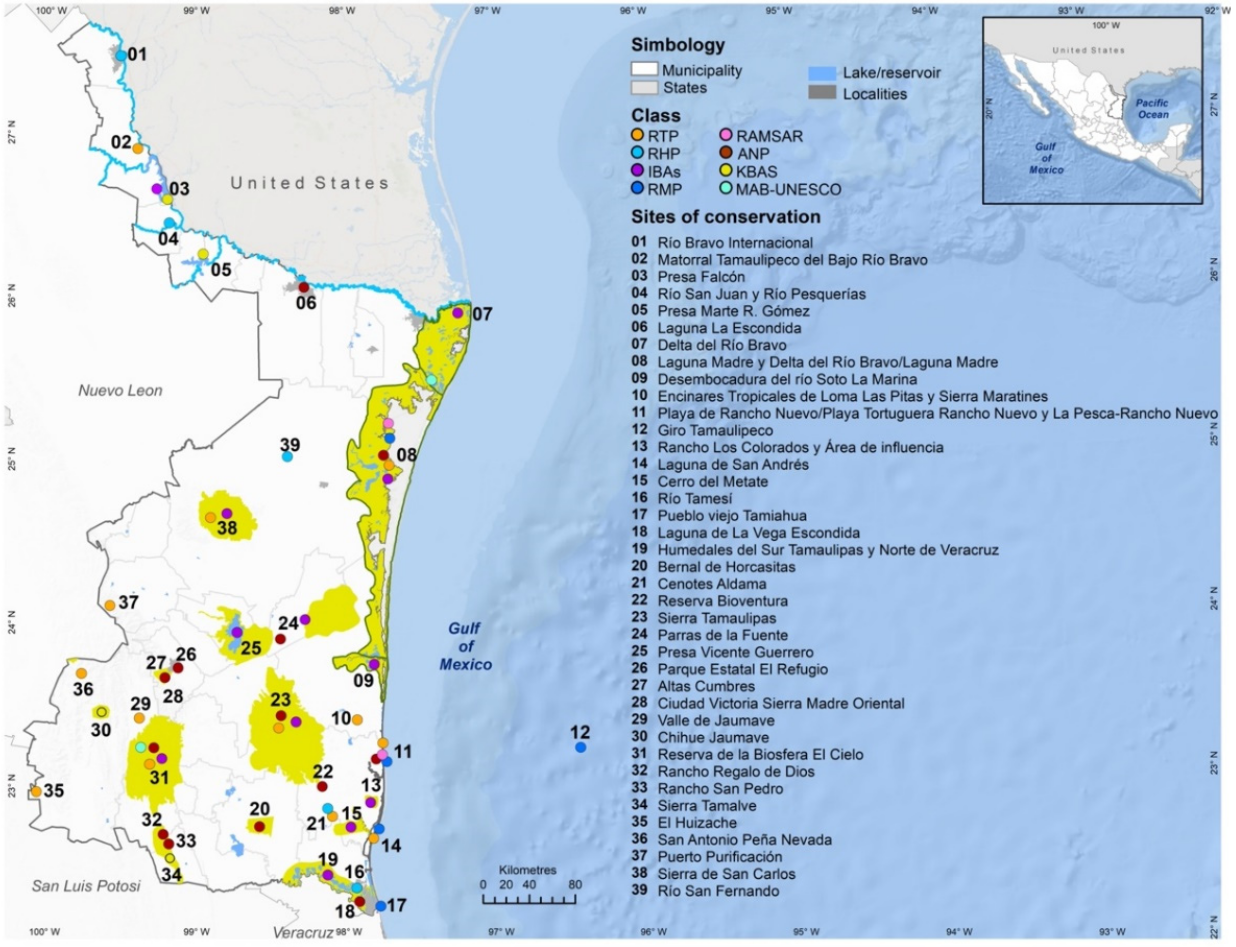
\includegraphics[width=1.00\linewidth]{figs/MapaTamps.png}\\
      \end{tabular}
\end{center}
\end{column} 
\end{columns} 
\footfullcite*{u14010494}
\end{frame}




% Tabla Areas protegidas vs Regiones
\frame{
\frametitle{Distribución de los sitios de conservación por region del estado de Tamaulipas }
\begin{columns}
\begin{column}{0.70\textwidth}
\begin{enumerate}
\item Fronteriza: 7
\item Valle de San Fernando: 2
\item Centro: 10
\item Altiplano: 4
\item El Mante: 4
\item Sur: 10
\item Oceánica: 1 (Giro Tamaulipeco)
\end{enumerate}
\textit{ADVC (Area destinada voluntariamente a la conservación). En Tamaulipas hay dos: Rancho San Pedro (Antiguo Morelos) y la Reserva Bio Ventura (Aldama) }
\end{column} 
\begin{column}{0.30\textwidth}

\begin{center}
% Fila1
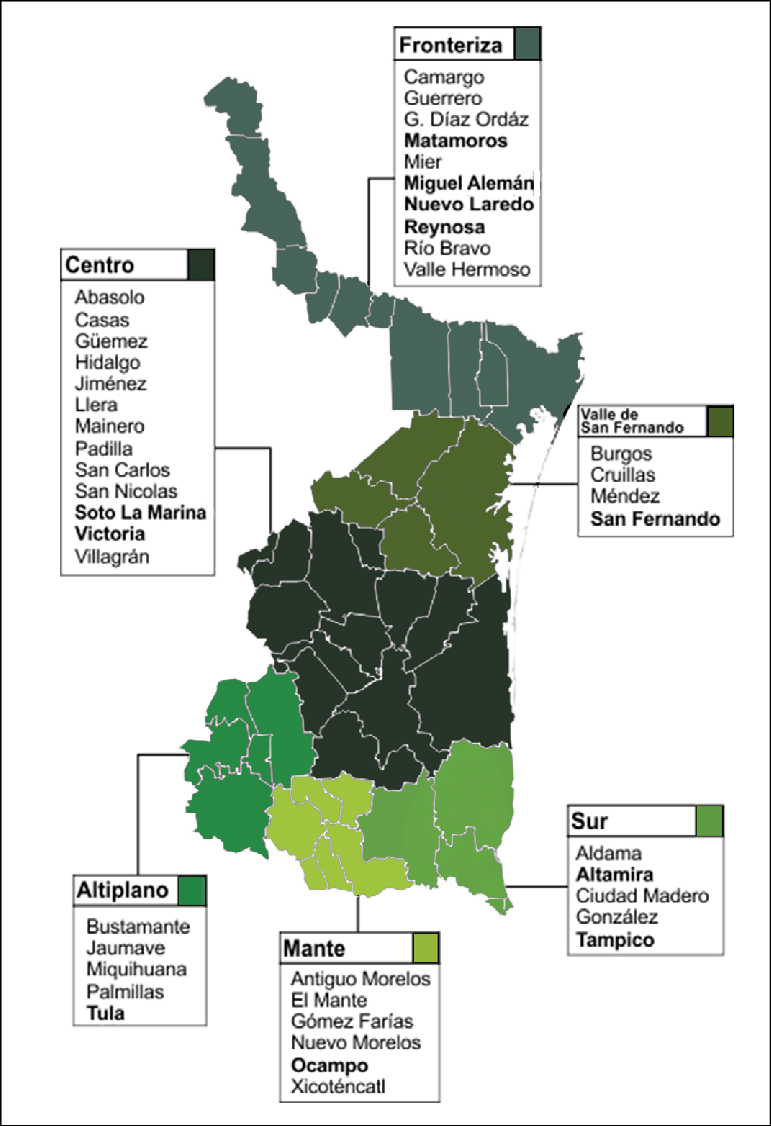
\includegraphics[width=1.00\linewidth]{figs/Figura-2-Regiones-de-Tamaulipas.png}\\
\end{center}
\end{column} 
\end{columns} 
}

% Tabla Areas protegidas vs Regiones
\frame{
\frametitle{Zona Oceánica Giro Tamaulipeco}
\begin{columns}
\begin{column}{0.85\textwidth}
\begin{enumerate}
\item AU: Áreas de uso por sectores
\item AFI: Áreas de falta de información de biodiversidad
\item Polígono: Latitud. 25°59'24'' a 20°33', Longitud. 97°19'48'' a 94°28'12''
\item Extensión: 90 145 km2
\item Oceanografía: como proceso oceánico está el Gran Giro Anticiclónico Tamaulipeco.
\item Biodiversidad: fitoplancton, zooplancton, peces, aves residentes (Laguna Madre) y aves migratorias.
\item Aspectos económicos: zona pesquera con conflictos internacionales (Zona Económica Exclusiva) y explotación de tiburón, atún y sardina.
\item Problemática: contaminantes industriales y petroleros.
\end{enumerate}
\end{column} 
\begin{column}{0.15\textwidth}

\begin{center}
% Fila1
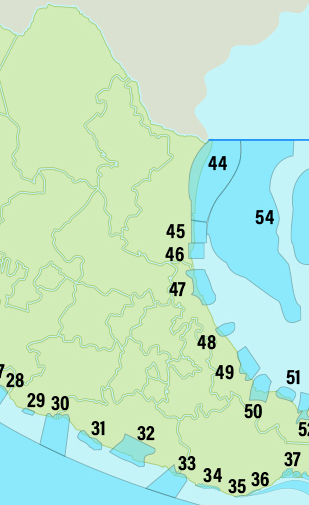
\includegraphics[width=1.00\linewidth]{figs/GiroTamaulipecoX.jpg}\\
\end{center}
\end{column} 
\end{columns} 
}






\section[MCAT]{Monitoreo de la Calidad del Agua en Tamaulipas}


\begin{frame}{Datos de la Red Nacional de Monitoreo de la Calidad de las Aguas Nacionales (RNMCA)}
\begin {itemize}
\item Se reportan datos de 4,561 sitios de monitoreo
\begin{itemize}
\item Aguas superficiales (3,493)
\item Aguas subterraneas (1,068)
\end{itemize}
\item Los datos disponibles son del año 2020
\item Con respecto al estado de Tamaulipas, sólo para aguas superficiales se tienen 164 sitios de monitoreo
\end{itemize}
\end{frame}

\begin{frame}{Parámetros de contaminación del agua}
Parámetros para determinar niveles de contaminación del AGUA:
\begin{itemize}
\item Chlorophyll-a (Chl-a)(Clorofila) - Medida de la cantidad de algas en el agua. Un exceso causa problemas en la cantidad de oxigeno disuelto,  además de que algunas pueden ser tóxicas
\item Turbidity (Turbiedad) - Medida de la claridad de un líquido
\item Total Suspended Matter (TSM) - Medida de la cantidad de sedimentos, que pueden ser de origen organico o inorgánico 
\item Secchi Disk Depth (SDD) - La profundidad Secchi se refiere a la profundidad a la que un disco sumergido en el agua ya no puede verse desde la superficie. La profundidad Secchi está relacionada con la claridad del agua y es una medida de la profundidad a la que puede penetrar la luz en el agua
\end{itemize}
\end{frame}


\frame{
\frametitle{Evaluación de la calidad del agua y del riesgo ecológico de los caudales intermitentes que atraviesan zonas mineras y urbanas de la subcuenca del río San Marcos, México}
\begin{columns}
\begin{column}{0.30\textwidth}
\begin{itemize}
\item Se analizó la calidad del agua y el riesgo ecológico en el sistema fluvial intermitente de El Novillo y San Marcos \cite{LOPEZ2020100369}$^*$
\end{itemize}
\end{column} 
\begin{column}{0.70\textwidth}
\begin{center}
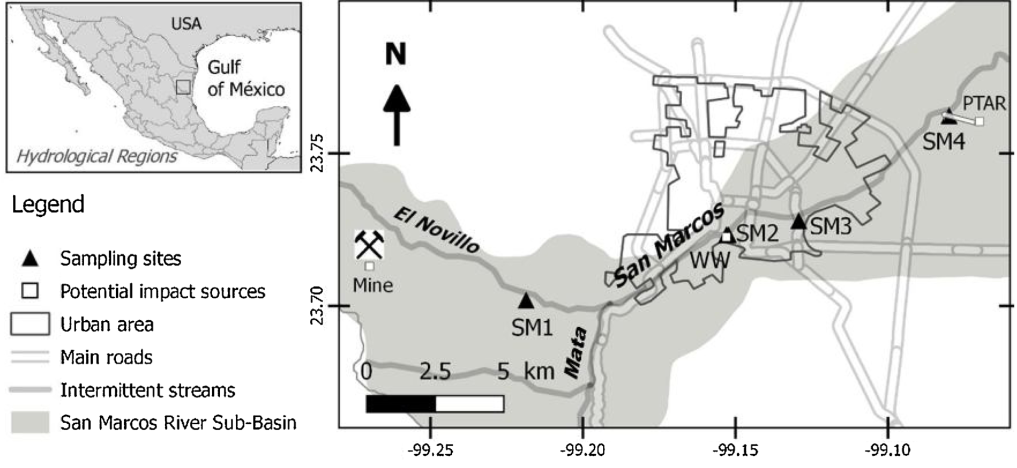
\includegraphics[width=1.00\linewidth]{figs/CalidadAguaVickyRanch.png}\\
\end{center}
\end{column}
\end{columns}
\footfullcite*{LOPEZ2020100369}
}

\frame{
\frametitle{Evaluación de la calidad del agua y del riesgo ecológico de los caudales intermitentes que atraviesan zonas mineras y urbanas de la subcuenca del río San Marcos, México}
%\begin{columns}
%\begin{column}{0.70\textwidth}
\begin{enumerate}
\item Se cuantificaron los contaminantes fisicoquímicos y microbiológicos 
\item En base a criterios criterios nacionales e internacionales, los promedios anuales de los parámetros de calidad del agua analizados sugieren que el caudal de estos sistemas fluviales es de mala calidad y supone un alto riesgo ecológico para la vida acuática.
\item En la zona urbana, las concentraciones medias anuales de Cd y Pb (0,14 y 0,4 mg/L) eran 77 y 10 veces superiores a sus respectivos criterios de calidad del agua (<0,0018 y 0,04 mg/L)
\end{enumerate}
}

% -- Hacerlo mediante un Arduino?
% Oportunidad: Implementar estaciones de monitoreo automáticas a prueba de condiciones meteorológicas extremas
% Problemas: Bandalismo, falta de recursos, etc

\begin{frame}{Integración de Sensado Remoto y datos de RMNCA (1)}

Integrar datos de la RMNCA y de imágenes satelitales \cite{s21124118}$^*$
\begin{itemize}
\item Datos de la Red Nacional de Monitoreo del Agua (2013–2019) 
\item Imágenes de Landsat-8 OLI, Sentinel-3 OLCI, and Sentinel-2 MSI 
\item Regiones estudiadas: Chapala, Cuitzeo, Pátzcuaro, Yuriria y Catemaco
\item Entrenamiento de diferentes clasificadores: extreme learning machine (ELM), support vector regression (SVR) y linear regression (LR)
\end{itemize}
\begin{center}
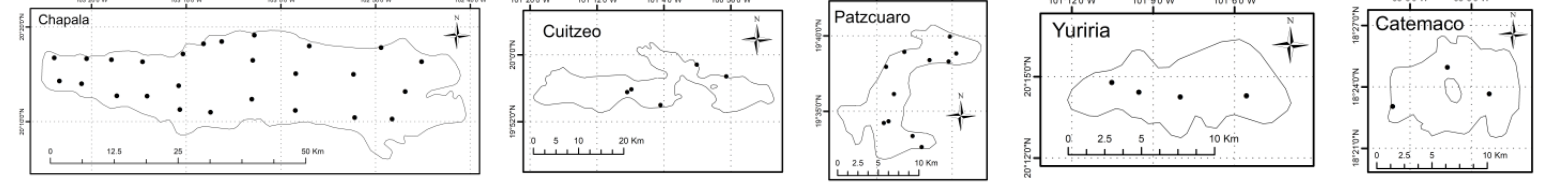
\includegraphics[width=1.00\linewidth]{figs/LagosMexico.png}\\
\end{center}


\footfullcite*{s21124118}
\end{frame}


\begin{frame}{Integración de Sensado Remoto y datos de RMNCA (2)}
\begin{itemize}
\item Operational Land Imager (OLI)
\item Ocean and Land Color Instrument (OLCI)
\item MultiSpectral Instrument (MSI)
\end{itemize}
Características de las imágenes satelitales utilizadas:
\begin{center}
\begin{tabular}{p{2.5cm}p{2.25cm}p{2.25cm}p{2.25cm}p{2.25cm}}
\hline
\hline
Satellite & Temporal Resolution (Days) & Spatial Resolution (m) & Launched & Spectral Bands \\
\hline
\hline
Landsat-8 OLI & 16 & 30 & 2013 & 11 \\ \hline
Sentinel-3A and 3B & 2-3 & 300 & 3A, 2016; 3B, 2018 & 21 \\ \hline
Sentinel-2A and 2B & 5 & 10 and 20 & 2A, 2015; 2B, 2017 11 & 13 \\
\hline
\hline
\end{tabular}
\end{center}


\end{frame}

\begin{frame}{Integración de Sensado Remoto y datos de RMNCA (3)}
\begin{center}
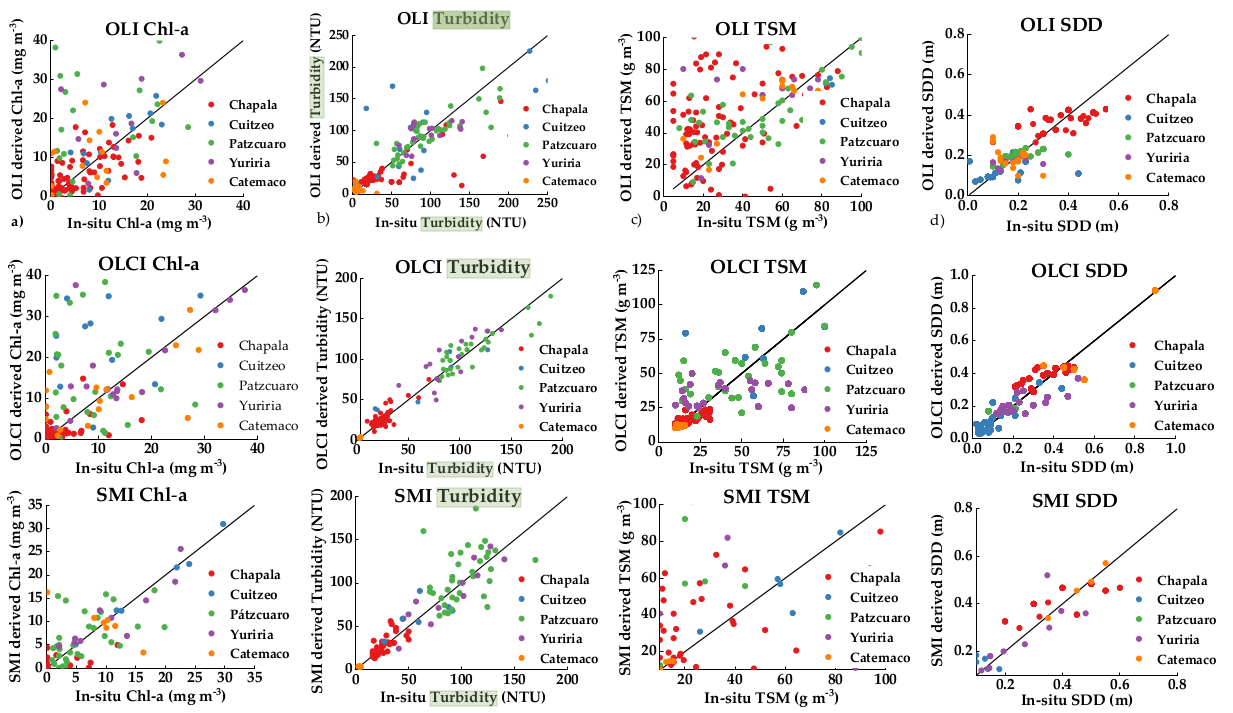
\includegraphics[width=0.80\linewidth]{figs/ParametrosContaminacion.png}\\
\end{center}
\end{frame}





%\section[CES]{Contaminantes en Especies Nativas}

\frame{
\frametitle{Evaluación de presencia de pesticidas en pescados de la presa Vicente Guerrero (1)}
\begin {itemize}
\item Se evaluó la presencia de pesticidas organoclorados (aldrín, endrín, clordano, mirex,
heptacloro, DDT, DDE, DDD) en el músculo de 4 especies de pescado de la Presa Vicente Guerrero del estado de Tamaulipas
(México): bagre; carpa, lobina  y tilapia \cite{72460107}$^*$
\item En México, la lista de los plaguicidas autorizados y restringidos se encuentra en el Catálogo Oficial de Plaguicidas, publicado por la Comisión Intersecretarial
para el Control y uso de Plaguicidas, Fertilizantes, y Sustancias Tóxicas (CICOPLAFEST)
\end {itemize}
\footfullcite*{72460107}
}


\frame{
\frametitle{Evaluación de presencia de pesticidas en pescados de la presa Vicente Guerrero (2)}
\begin{itemize}
\item Para la determinación de los pesticidas se usó extracción en fase sólida y cromatografía de gases con detector de
captura de electrones
\item 5 ejemplares para cada especie, ng/g, desviación estándar entre paréntesis, DLD (Debajo del límite de detección)
\item El p,p'-DDE es un metabolito y producto de degradación del pesticida organoclorado DDT (Dichlorodiphenyltrichloroethane)
\end{itemize}

\begin{center}
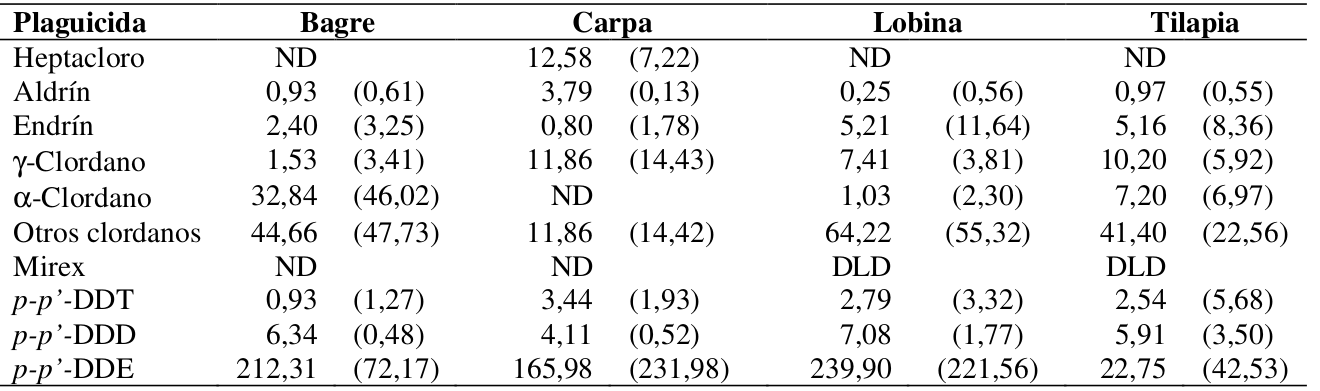
\includegraphics[width=0.80\linewidth]{figs/PlaguicidasPresaVicenteGuerrer.png}\\
\end{center}
}




\section[CFFT]{Caracterización de Flora y Fauna en Tamps}
%

\frame{
\frametitle{Diversity, distribution and conservation of the Cactaceae (Caryophyllales) from Tamaulipas, Mexico (1)}

\begin{itemize}
\item Se utilizaron bases de datos para generar una distribución geográfica, diversidad, endemismo y conservación de las Cactaceae en Tamaulipas \cite{doi:10.1080/11263504.2022.2056648}$^*$
\item El territorio de Tamaulipas se dividió en celdas cuadriculadas de 10 × 10 minutos latitud/longitud y se utilizaron como unidades de análisis \footnote{Un minuto equivale a 1,8 Km}
\item La mayor diversidad de especies se da en la región suroccidental asociada a las laderas de la Sierra Madre Oriental y el valle de Jaumave
\end{itemize}


%\textit{Un taxón o taxon es un grupo de organismos emparentados​} %, que en una clasificación dada han sido agrupados, asignándole al grupo un nombre en latín, una descripciín si es una especie, y un tipo}
%\textit{Un taxón o taxon es un grupo de organismos emparentados, que en una clasificación dada han sido agrupados, asignándole al grupo un nombre en latín, una descripción si es una especie, y un tipo}
%\url{https://www.tandfonline.com/doi/full/10.1080/11263504.2022.2056648?scroll=top&needAccess=true&role=tab}


\footfullcite*{doi:10.1080/11263504.2022.2056648}
}




\frame{
\frametitle{Diversity, distribution and conservation of the Cactaceae (Caryophyllales) from Tamaulipas, Mexico (2)}
\begin{columns}
\begin{column}{0.60\textwidth}
\begin{itemize}
\item Revisaron 25 años de registros en diferentes herbarias (por ejemplo, Univ de Arizona)
\item Bases de datos de las CONABIO y del Missouri Botanical Garden
\item Se obtuvieron 3698 registros con coordenadas geograficas incluidas 
\end{itemize}
\end{column} 
\begin{column}{0.50\textwidth}
\begin{center}
% Fila1
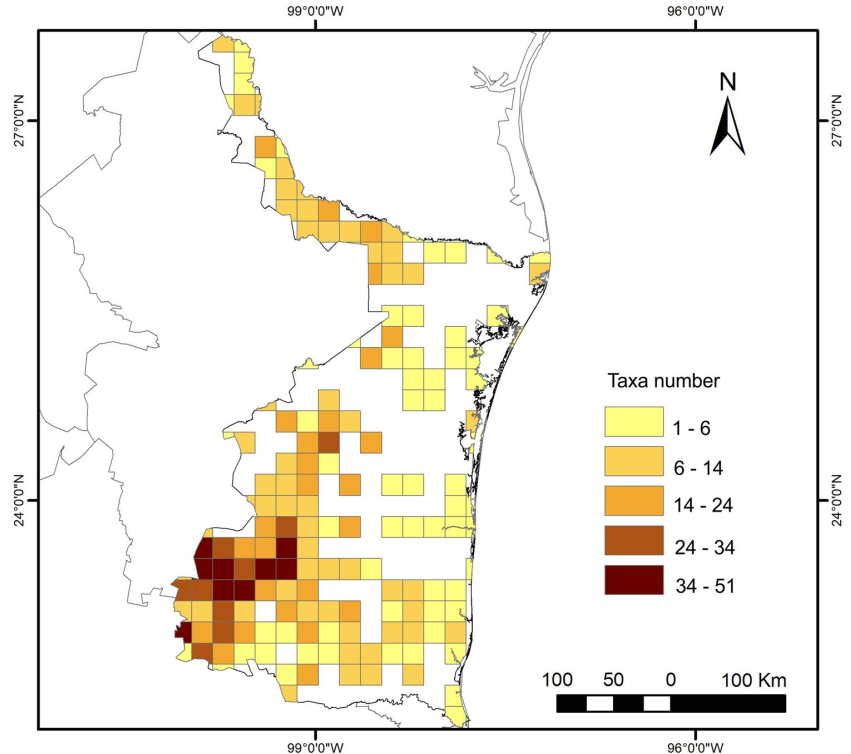
\includegraphics[width=1.00\linewidth]{figs/GridCells.png}\\
\end{center}
\end{column} 
\end{columns}
}

%\section[SIG]{Uso de SIGs para obtener información ambiental}

\frame{
\frametitle{SIG y Google Earth para modelo de distribución del bosque de oyamel en Tamaulipas (1)}
\begin{itemize}
\item En la parte septentrional de México los Oyamel (Abetos) son escasos y restringidos. 
\item En Tamaulipas se ubican cercanos al Cerro San Antonio Peña Nevada, que forma parte la Sierra Madre Oriental
\item Los mapas actuales de distribución de las comunidades vegetales mexicanas, como los de INEGI, se encuentran disponibles en formato digital a una escala de 1:250,000 \cite{articleOchoa2015}$^*$
\end{itemize}
\footfullcite*{articleOchoa2015}
}

\frame{
\frametitle{SIG y Google Earth para modelo de distribución del bosque de oyamel en Tamaulipas (2)}

\begin{itemize}
\item El área mínima cartografiable es mayor al tamaño de relictos de oyamel observados en Tamaulipas, situados en algunas cañadas y cerros, con individuos de Abies formando bosquecillos, que no se han registrado oficialmente 
\item Se utilizó el módulo Spatial Analyst para el software ArcView, que a partir de mapas en formato raster  para determinar la presencia de la especie en los mapas 
\item El área de estudio se restringe a los sitios con elevación igual o superior a los 2,500 msnm
\item En el municipio de Miquihuana existen elevaciones mayores a 3,000 msnm, por lo que en este municipio se visitó un sitio previamente identificado con presencia de Abies, (Cerro del Nacimiento), donde el bosquecillo fue encontrado a 3,200 msnm.
\end{itemize}
}

\frame{
\frametitle{SIG y Google Earth para modelo de distribución del bosque de oyamel en Tamaulipas (3)}
\begin{center}
% Fila1
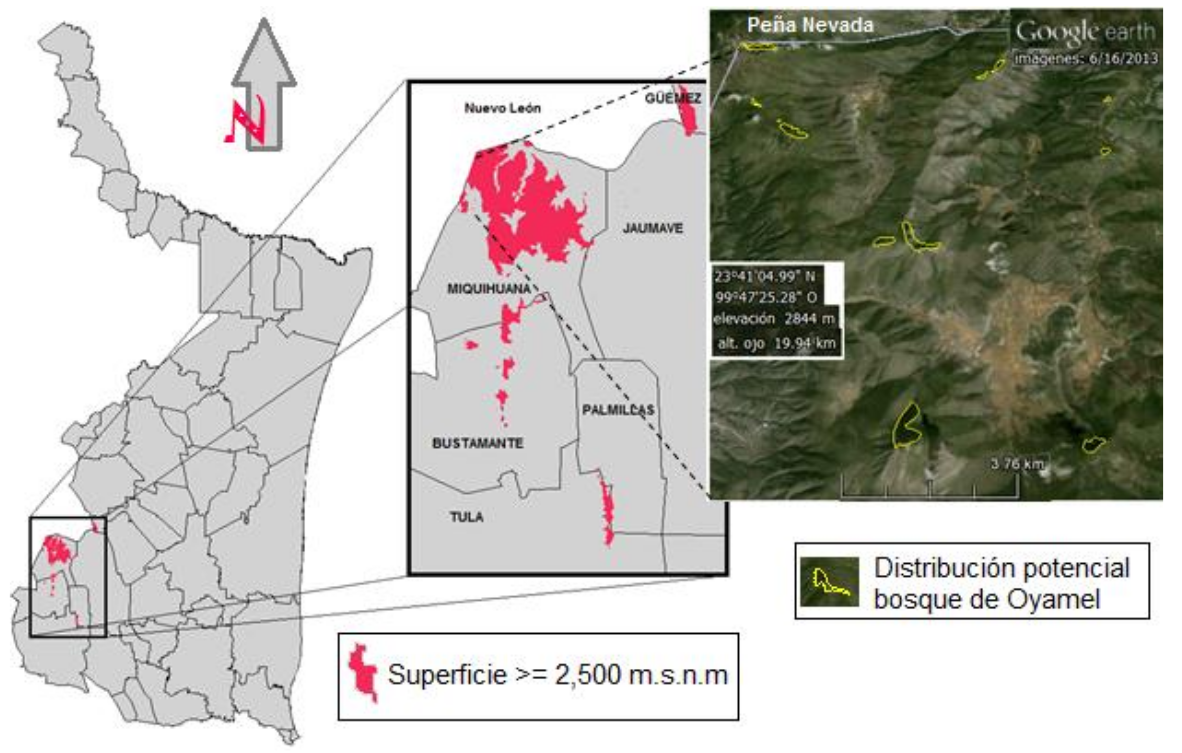
\includegraphics[width=0.70\linewidth]{figs/OyamelesTamsp.png}\\
\end{center}
}



%\section[MF]{Monitoreo del Felinos}

\frame{
\frametitle{Análisis paisajístico del hábitat del jaguar (Panthera onca) (1)}
\begin{itemize}
\item Se empleo un SIG para evaluar la influencia de las actividades humandas en la estructura del habitat del Jaguar (panthera onca) en la Sierra de Tamauliopas \cite{ortega-huerta_medley_1999}$^*$ 
\item En dicho estudio:
\begin{itemize}
\item Se clasificó el hábitat potencial en función de las asociaciones entre entre los atributos medioambientales (topografía
y vegetación) y la distribución de frecuencia de
registros de avistamientos de jaguares; 
\item Se clasificó la cobertura de una imagen Landsat-TM de 1990 y mapeó la estructura
la estructura del paisaje del hábitat de alto potencial; 
\item Se comparó el grado de fragmentación de la vegetación fragmentada por diferentes tipos de propietarios.
\end{itemize}
\end{itemize}
\footfullcite*{ortega-huerta_medley_1999}
}

\frame{
\frametitle{Análisis paisajístico del hábitat del jaguar (Panthera onca) (2)}
\begin{center}
\begin{tabular}{cc}
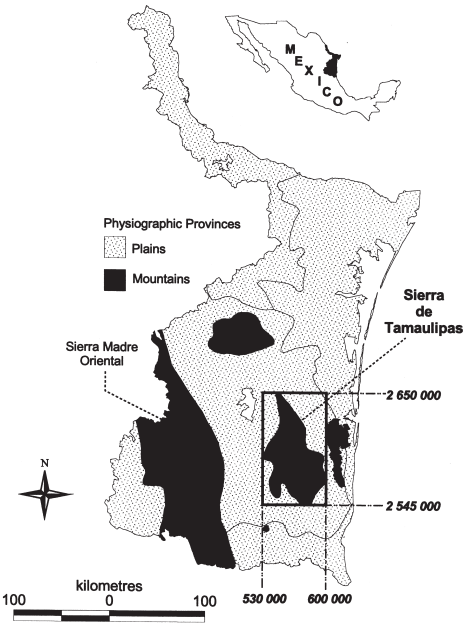
\includegraphics[width=0.25\linewidth]{figs/SierraTamps.png} &  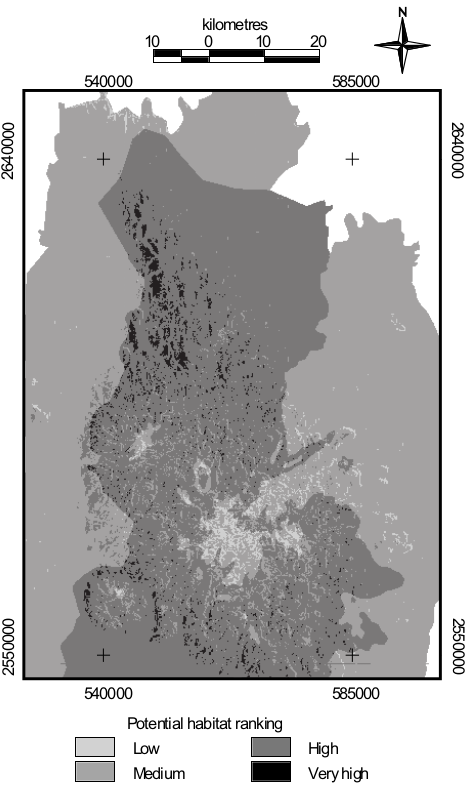
\includegraphics[width=0.25\linewidth]{figs/SierraTamulipasJaguar.png} \\
\end{tabular}
\end{center}
}





\frame{
\frametitle{Confirmación de jaguares, ocelotes y jaguarundis en la Sierra de San Carlos (1)}
\begin{itemize}
%\item \cite{10.1093/jmammal/gyab134}$^*$ 
\item El área de distribución del jaguar, ocelote y jaguarundi en el noreste de México no está bien reconocida 
\item La Sierra de San Carlos (24°30' \& 25°00' N / 98°30' \& 99° 15' O) también conocida como Sierra Chiquita o Cruillas, esta ubicada en el norte del tamaulipas
\item No hya registros confirmado de estas especies dentro de la Sierra de San Carlos, aunque en estudios previos se incluye esta área como potencial para la
la distribución de las tres especies de felinos
\item En un artículo \cite{caso2018confirmed}$^*$ se confirma fotográficamente la visita de ocelotes y jaguarundis en un ojo de agua dentro del Rancho Sílica, y posteriormente también fue confirmada la visita de un jaguar en el mismo lugar
\end{itemize}
%\footfullcite*{10.1093/jmammal/gyab134}
\footfullcite*{caso2018confirmed}

}

\frame{
\frametitle{Confirmación de jaguares, ocelotes y jaguarundis en la Sierra de San Carlos (2)}
\begin{center}
\begin{tabular}{cc}
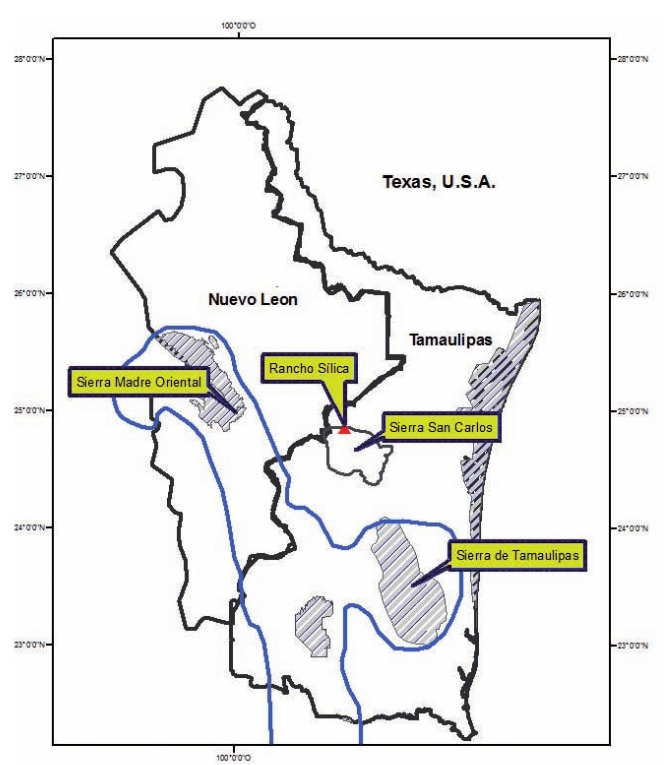
\includegraphics[width=0.35\linewidth]{figs/JaguarOceloteJaguarundi1.png} &  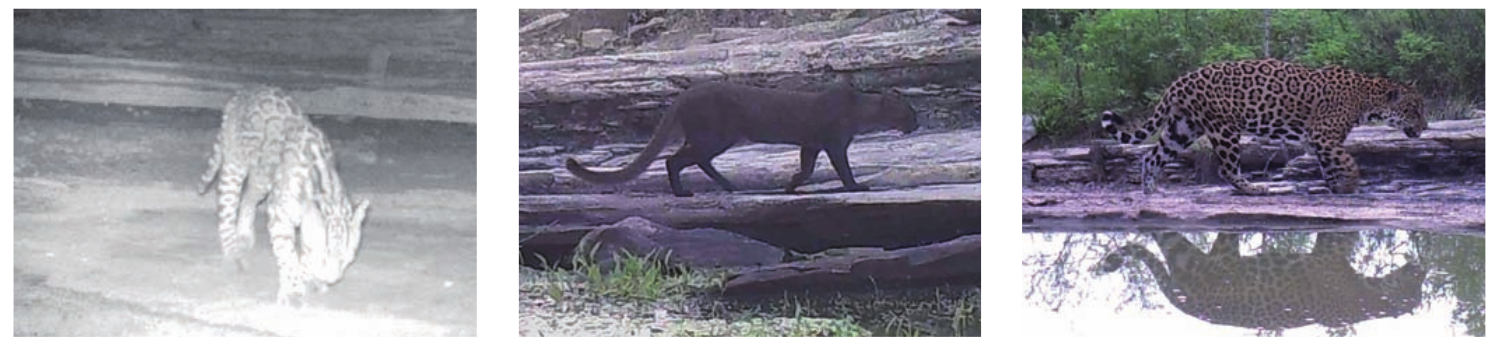
\includegraphics[width=0.60\linewidth]{figs/JaguarOceloteJaguarundi2.png} \\
\end{tabular}
\end{center}
}



\frame{
\frametitle{Estimación de la densidad de población del Ocelote (1) }
\begin{itemize}
\item Se realizó una estimación del Ocelote (Leopardus pardali) en la región de la Laguna Madre, Tamaulipas \cite{OcanasJaguares}$^*$ 
\item Se obtuvieron 473 registros fotográficos, identificando 51 individuos (19 machos, 19 hembras, 13 no identificados)
\item Se utilizarón dos herramientas software para estimar la densidad poblacional (CAPTURE y SPACECAP) a partir de los datos del fototrampeo
\item Atribuyen la alta densidad de ocelotes a la ausencia del jaguar (Pantera orca)
\end{itemize}

\footfullcite*{OcanasJaguares}
}

\frame{
\frametitle{Estimación de la densidad de población del Ocelote (2)}
\begin{center}
\begin{tabular}{cc}
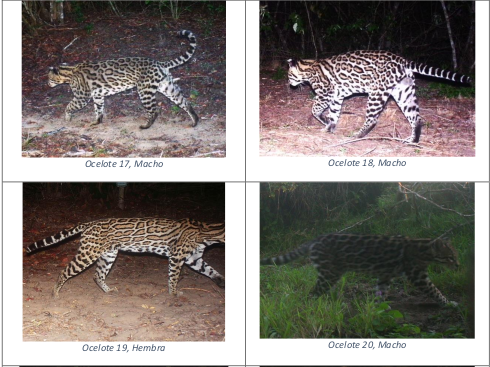
\includegraphics[width=0.50\linewidth]{figs/Ocelotes1.png} &  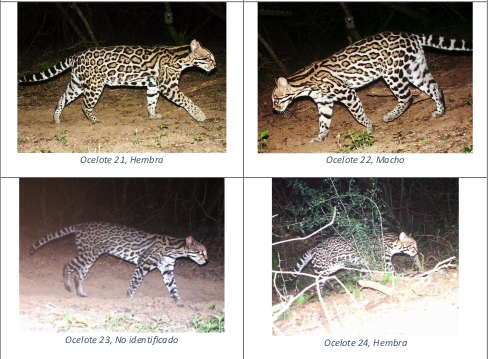
\includegraphics[width=0.50\linewidth]{figs/Ocelotes2.png} \\
\end{tabular}
\end{center}
}



\frame{
\frametitle{Monitoreo jaguarundi (1)}
\begin{itemize}
\item Se realizó un censo de 2003 a 2021 utilizando cámaras-trampa en el sur de Texas y el norte de Tamaulipas, México, con el fin de estudiar las poblaciones de felinos medianos (ocelotes [Leopardus pardalis], linces [Lynx rufus] y jaguares) \cite{doi.org/10.1002/ece3.8642}$^*$ 
\item El último avistamiento de un jaguarundi en Texas fue en 1986 (atropellado)
\item Después de 350,366 noches trampa en 685 sitios con cámaras, no se detectaron jaguarundis en 16 propiedades o a lo largo de 2 carreteras (1050 km$^2$ ) en Texas. 
\item Sin embargo, se registrarón 126 detecciones fotográficas de jaguaruarundi en 15,784 noches trampa en 2 propiedades (125.3 km$^2$ ) en la Sierra Norte de Tamaulipas.
la Sierra Norte de Tamaulipas, Tamaulipas, México 
\end{itemize}
\footfullcite*{doi.org/10.1002/ece3.8642}
}

% Oportunidad: Un sistema basado en Raspberry-Pi, Ardunio
% Indentificar multiples especies?

\frame{
\frametitle{Monitoreo jaguarundi (2)}
\begin{center}
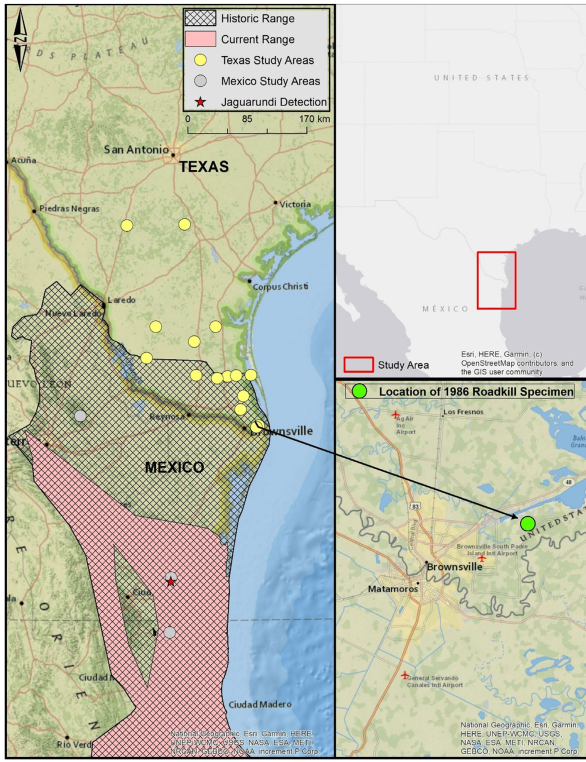
\includegraphics[width=0.35\linewidth]{figs/JaguarundiTexasMexico.png}
\end{center}
}






\frame{
\frametitle{Comparación de sistemas para diferenciar Ocelores de Jaguares (1) }
\begin{itemize}
\item Se utilizaron 2 conjuntos de imágenes de cámaras trampa: 359 imágenes de jaguares (Panthera onca) y 332 imágenes de ocelotes (Leopardus pardalis) 
\item Las imagenes fueron obtenidas de cámaras trampa desplegadas en 4 lugares de estudio en el Orange Walk, Belice, en 2015 y 2016 
\item Se compararon la precisión de HotSpotter y Wild-ID, y evaluar el efecto de la calidad de la imagen en el éxito del emparejamiento. 
\cite{articleNipko2020}$^*$ 
\end{itemize}
\footfullcite*{articleNipko2020}
}

\frame{
\frametitle{Comparación de sistemas para diferenciar Ocelores de Jaguares (2) }
\begin{itemize}
\item En general, HotSpotter seleccionó una correcta como su rango superior en un 71-82\% de las ocasiones, mientras que la tasa de Wild-ID fue del 58-73\%.
\end{itemize}

\begin{center}
\begin{tabular}{cc}
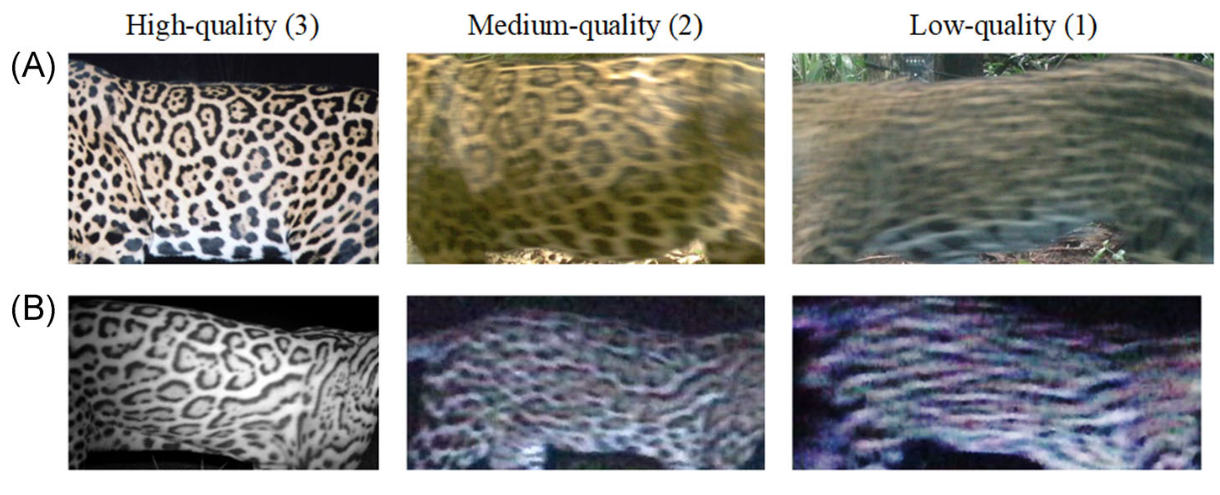
\includegraphics[width=0.50\linewidth]{figs/JaguarsyOcelots1.png} &  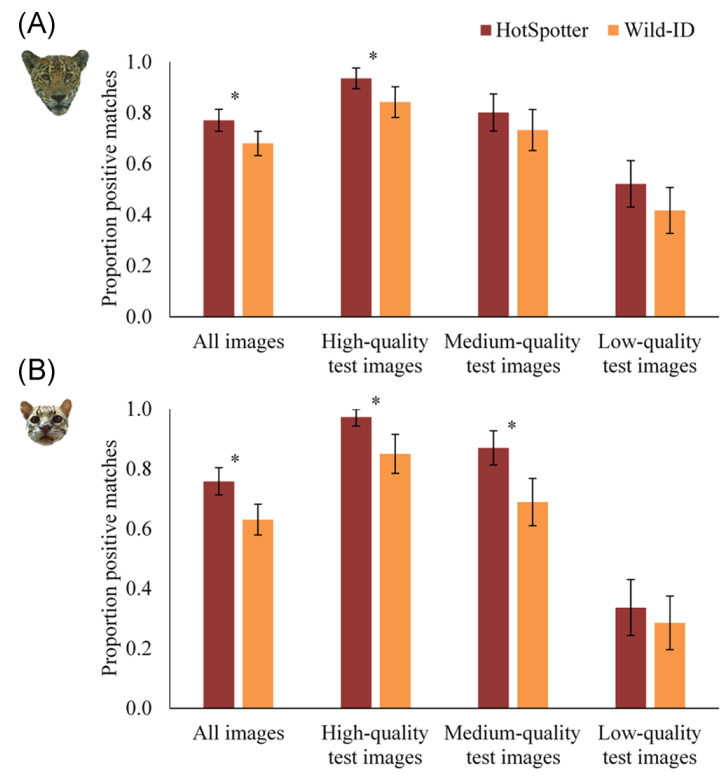
\includegraphics[width=0.30\linewidth]{figs/JaguarsyOcelots2.png} \\
\end{tabular}
\end{center}
}















\section[SEMs]{Monitoreo Ambiental Inteligente}

\begin{frame}{Monitoreo Ambiental y Monitoreo Ambiental Inteligente (1)}
	\begin{itemize}  %del cuerpo académico Acuicultura Sustentable (UTMTB-CA-1)
		\item \textit{``El monitoreo ambiental (EM por sus siglas en inglés) consiste en planificar y gestionar adecuadamente las catástrofes, controlar las distintas contaminaciones y afrontar eficazmente los retos que surgen debido a condiciones externas insalubres. El EM se ocupa de la contaminación del agua, el aire, las radiaciones peligrosas, los cambios meteorológicos, los terremotos, etc. '' \cite{s20113113}$^*$}
		\item \textit{``Con los avances recientes de la ciencia y la tecnología, especialmente la inteligencia artificial (IA) y el aprendizaje automático, el EM se ha convertido en un sistema de monitoreo ambiental inteligente (SEM por sus siglas en inglés), porque la tecnología ha permitido que los métodos de EM vigilen con mayor precisión los factores que inciden en el medio ambiente, con un control óptimo de la contaminación y otros efectos indeseables''}
	\end{itemize}
\footfullcite*{s20113113}
\end{frame}


\begin{frame}{Monitoreo Ambiental (EM) y Monitoreo Ambiental Inteligente (SEM) (2)}
Los SEMs se pueden categorizar en las siguientes clases:
\begin{itemize}
\item Sistemas inteligentes de monitoreo de la agricultura (SAMs) 
\item Sistemas inteligentes de monitoreo de la contaminación del agua (SWPMs)
\item Sistemas inteligentes de monitoreo del aire (SAQMs)
\end{itemize}
En las categorias anteriores se incluyen:  Monitoreo del suelo (SM), del medio oceánico (OEM), del medio marino (MEM), de la calidad del aire
(AQM), de la calidad del agua (WQM) y de la radiación (RM).
\end{frame}


\begin{frame}{Sistemas SM, OEM, MEM, AQM, WQM y RM (1)}
\begin{center}
\footnotesize
\begin{tabular}{p{4.5cm}|p{4.5cm}|p{4.5cm}}
\hline
\textbf{Propósito} & \textbf{Ventajas/Desafíos} & \textbf{Metodos/Dispositivos} \\
\hline
Vigilancia del entorno oceánico  &
Peso ligero; redes sensoriales costosas e invasivas &  
Sensores inalámbricos \\ \hline

Monitorización del suelo para la agricultura & 
Monitorización eficiente de cultivos de hortalizas; los gases de efecto invernadero afectan a la salud de hortalizas como el tomate & 
Sensores inalámbricos \\  \hline


Monitorización acústica del entorno marino &
Menor latencia; bajo consumo de energía; problemas de instalación y cobertura &
WSN e IoT \\  \hline


Sistema de monitorización de la contaminación atmosférica &
Kit móvil ``IoT-Mobair'' para predicción; precisión inferior; baja sensibilidad; computacionalmente complejo  &
Sensor de gas e IoT \\  \hline

\end{tabular}
\end{center}

\end{frame}


\begin{frame}{Sistemas SM, OEM, MEM, AQM, WQM y RM (2)}
\begin{center}
\footnotesize
\begin{tabular}{p{4.5cm}|p{4.5cm}|p{4.5cm}}
\hline
\textbf{Propósito} & \textbf{Ventajas/Desafíos} & \textbf{Metodos/Dispositivos} \\
\hline

Monitorización de la calidad del aire &
Monitorización de la calidad del aire escalable y de alta densidad con interconexión de sensores heterogéneos; complejidad computacional debido a los enormes datos capturados y procesados &
Red de sensores móviles y WSN  \\  \hline

Monitorización medioambiental &
Norma W3C de interoperabilidad; problemas de interoperabilidad de sensores heterogéneos &
Sensores heterogéneos \\  \hline

Monitorización de la calidad del aire &
Supervisión de grandes áreas; datos ruidosos; problemas de precisión y coste &
Sensores geomáticos e IoT \\  \hline

Monitorización de la contaminación del aire &
Sistema Monitorización en tiempo real; problemas de precisión  &
Sensores con modelo MQ3, Raspberry Pi e IoT \\  \hline


\end{tabular}
\end{center}

\end{frame}

\begin{frame}{Sistemas SM, OEM, MEM, AQM, WQM y RM (3)}
\begin{center}
\footnotesize
\begin{tabular}{p{4.5cm}|p{4.5cm}|p{4.5cm}}
\hline
\textbf{Propósito} & \textbf{Ventajas/Desafíos} & \textbf{Metodos/Dispositivos} \\
\hline

Sistema de monitorización de la contaminación del aire  &
Eficiente para áreas de baja cobertura; bajo coste; fácil de instalar; se cubre un menor número de contaminantes &
Sensor de gas y sensor LASER \\  \hline

Vigilancia del polvo y la humedad &
Amplia cobertura y eficiencia; bajo coste y pequeño tamaño &
IoT \\  \hline

Monitorización de la radiación &
Alto coste y baja estabilidad frente a variaciones de temperatura &
Cámara HPXe \\  \hline

Acuicultura &
Control de la calidad y cantidad del agua; mayor emisión de carbono y necesidad de energía &
Sensor de olor, pH, conductancia y temperatura \\  \hline

Efecto del entorno sólo en invierno &
Efecto de las baterías y otras radiaciones &
Red de sensores inalámbricos \\  \hline



\end{tabular}
\end{center}

\end{frame}


\begin{frame}{Sistemas SM, OEM, MEM, AQM, WQM y RM (4)}
\begin{center}
\footnotesize
\begin{tabular}{p{4.5cm}|p{4.5cm}|p{4.5cm}}
\hline
\textbf{Propósito} & \textbf{Ventajas/Desafíos} & \textbf{Metodos/Dispositivos} \\
\hline

Sistema de supervisión de la salud electrónica debido a los cambios de temperatura y radiación en el entorno &
Detección de situaciones de emergencia &
Sistema de supervisión e IA \\  \hline

Vigilancia del clima y la ecología &
Estudio de las emisiones en el entorno &
Tecnología LoRa y red de sensores \\  \hline

Monitorización de la radiación en centros de datos &
Temperatura, humedad y consumo de energía en centros de datos monitorizados para ciudad inteligente y SEM &
IoT \\  \hline

Entorno industrial inteligente &
Estudiar efectos peligrosos en industrias &
ZigBee y WSN LoRa: Largo alcance \\  \hline


\end{tabular}
\end{center}

\end{frame}


\begin{frame}{Sistemas para SAM (1)}
\begin{center}
\footnotesize
\begin{tabular}{p{4.5cm}|p{4.5cm}|p{4.5cm}}
\hline
\textbf{Propósito} & \textbf{Metodos/Dispositivos} & \textbf{Modelos} \\
\hline

Crecimiento de las plantas &
IoT, WSN, aprendizaje automático basado en ``gCrop'' (cultivo verde) &
Modelo de regresión de 3er grado de polinomio con una precisión de predicción del 98\%, pero adolece de complejidad computacional \\  \hline

Calidad de los cultivos &
SVM utilizando radar de apertura sintética (SAR) de teledetección para el seguimiento del arroz con cáscara &
Características de retrodispersión, SVM y árbol de regresión con una precisión del 77,65\%; tamaño de muestra limitado \\  \hline

Índice de área foliar &
Imágenes SAR y aprendizaje automático y SVM &
Modelo de proceso gaussiano, tamaño de muestra limitado \\  \hline

Área de cultivo &
Aprendizaje profundo para la monitorización de la superficie vegetal del cultivo de cacahuate &
CNN con 96,45\% de precisión\\  \hline

\end{tabular}
\end{center}

\end{frame}

\begin{frame}{Sistemas para SAM (2)}
\begin{center}
\footnotesize
\begin{tabular}{p{4.5cm}|p{4.5cm}|p{4.5cm}}
\hline
\textbf{Propósito} & \textbf{Metodos/Dispositivos} & \textbf{Modelos} \\
\hline

Calidad de los cultivos &
Aprendizaje automático aplicado a imágenes de UAV en tiempo real del cultivo de soja. Se probaron 5 enfermedades diferentes y se evaluó la calidad del suelo &
Resnet-50, VGG-19 con una precisión del 99,04 \\  \hline

Calidad de los cultivos &
Aprendizaje profundo aplicado sobre datos fenológicos, se probaron 6 cultivos diferentes &
CNN (red neuronal convolucional), precisión no mencionada \\  \hline

Agricultura inteligente &
IoT, WSN, aprendizaje profundo para el crecimiento de la fruta &
SVM, precisión no mencionada \\  \hline

Control de plagas &
IoT y aprendizaje profundo utilizando características globales y locales para el control de plagas &
Modelo CNN con un 86,6\% de precisión media \\  \hline




\end{tabular}
\end{center}

\end{frame}


\begin{frame}{Sistemas para SWPMs (1)}
\begin{center}
\footnotesize
\begin{tabular}{p{4.5cm}|p{4.5cm}|p{4.5cm}}
\hline
\textbf{Propósito} & \textbf{Metodos/Dispositivos} & \textbf{Modelos} \\
\hline

Control de la contaminación del agua agrícola mediante teledetección &
Aprendizaje automático y análisis de imágenes para la predicción &
Regresión lineal (LR), descenso de gradiente estocástico (SGD) y regresión de cresta (R-23 PLS)\\  \hline

Evaluación de la contaminación del agua &
FFT y aprendizaje automático &
Descriptor de disposición del color y SVM \\  \hline

Estudio de contaminantes del agua &
Aprendizaje extremo Modelo DSA-ELM para clasificación  &
Modelo DSA-ELM y enjambre de delfines con un 83,33\% de precisión \\  \hline

Análisis de la contaminación del agua &
Red neuronal para la predicción de los valores de alcalinidad, cloruro y sulfato &
Algoritmo Levenberg-Marquardt con 87,23\% de precisión \\  \hline

\end{tabular}
\end{center}

\end{frame}


\begin{frame}{Sistemas para SWPMs (2)}
\begin{center}
\footnotesize
\begin{tabular}{p{4.5cm}|p{4.5cm}|p{4.5cm}}
\hline
\textbf{Propósito} & \textbf{Metodos/Dispositivos} & \textbf{Modelos} \\
\hline

Análisis de la contaminación del agua &
Clasificación basada en aprendizaje automático &
SVM con una precisión del 91,38\%  \\  \hline

Análisis de agua potable &
Aprendizaje automático para clasificación: agua potable o no potable &
DT, KNN, SVM con 97\% de precisión  \\  \hline

Análisis de la contaminación del agua &
Red neuronal para clasificación: agua potable o no potable &
SVM \\  \hline

Vigilancia de la contaminación del agua &
SVM para clasificación como agua contaminada o limpia &
SVM con una precisión del 93,8\%  \\  \hline

Análisis del agua potable &
Predicción basada en aprendizaje automático &
Técnica de aprendizaje FAST \\  \hline

\end{tabular}
\end{center}

\end{frame}


\begin{frame}{Sistemas para SWPMs (3)}
\begin{center}
\footnotesize
\begin{tabular}{p{4.5cm}|p{4.5cm}|p{4.5cm}}
\hline
\textbf{Propósito} & \textbf{Metodos/Dispositivos} & \textbf{Modelos} \\
\hline

Concentración de clorofila-A en agua de lago &
Clasificación del agua basada en aprendizaje automático &
BPNN, SVM con 78 \% de precisión \\  \hline

Monitorización de la calidad del agua &
IoT para la evaluación de la calidad del agua superficial &
IoT con sensores inteligentes \\  \hline

\end{tabular}
\end{center}

\end{frame}


\begin{frame}{Sistemas para SAQMs (1)}
\begin{center}
\footnotesize
\begin{tabular}{p{4.5cm}|p{4.5cm}|p{4.5cm}}
\hline
\textbf{Propósito} & \textbf{Metodos/Dispositivos} & \textbf{Modelos} \\
\hline

Caracterización de la calidad del aire &
Monitorización de la calidad del aire &
Sensores heterogéneos; modelo predictivo basado en aprendizaje automático \\  \hline

Modelización de la calidad del aire &
Monitorización de la calidad del aire & 
Nodos móviles \\  \hline

Contaminación del aire &
Monitorización de la calidad del aire &
Sensores de gas a partir de datos de vehículos móviles, IoT y aprendizaje automático \\  \hline

Calidad del aire en red de sensores vehiculares &
Monitorización de la calidad del aire &
Sensores en nodos móviles \\  \hline

Detección de COV en el aire &
Detección de compuestos orgánicos &
Sensores infrarrojos, espectroscopia y aprendizaje automático \\  \hline


\end{tabular}
\end{center}

\end{frame}


\begin{frame}{Sistemas para SAQMs (2)}
\begin{center}
\footnotesize
\begin{tabular}{p{4.5cm}|p{4.5cm}|p{4.5cm}}
\hline
\textbf{Propósito} & \textbf{Metodos/Dispositivos} & \textbf{Modelos} \\
\hline

Estimación de PM2,5 &
Calidad del aire en términos de niveles de concentración de PM2,5 &
Datos geográficos espaciotemporales, técnica de aprendizaje automático extremo \\  \hline

Aire urbano & 
Contaminación del aire urbano en términos de concentraciones de O3, NO2 y SO2 &
Modelos de predicción \\  \hline

Predicción de la contaminación atmosférica &
Control de la contaminación atmosférica &
RFID, sensores de gas e IoT \\  \hline

Calidad del aire inteligente & 
Calidad del aire &
Sensor de temperatura, humedad, polvo y dióxido de carbono; LoRaWAN \\  \hline

Sistema inteligente de calidad del aire &
Calidad del aire para la detección de CO2, NOx, temperatura y humedad &
Luz UV, AI y sensores \\  \hline

\end{tabular}
\end{center}

\end{frame}

\begin{frame}{Sistemas para SAQMs (3)}
\begin{center}
\footnotesize
\begin{tabular}{p{4.5cm}|p{4.5cm}|p{4.5cm}}
\hline
\textbf{Propósito} & \textbf{Metodos/Dispositivos} & \textbf{Modelos} \\
\hline

Ozono, PM10 y PM2,5 &
PM10, PM2,5, SO2, óxidos de nitrógeno (NOx), O3, plomo, CO y benceno &
Aprendizaje automático y datos espaciotemporales  \\  \hline

Calidad del aire &
Calidad del aire  &
Sensores heterogéneos y SVM  \\  \hline

O3 anormal &
Ozono (O3) &
Datos de ozono y aprendizaje profundo  \\  \hline

Sensores portátiles &
Monitorización de temperatura y humedad &
Tecnología de sensores inalámbricos y wearables  \\  \hline

Monitorización de CO2 &
Monitorización del dióxido de carbono &
IoT y tecnologías en la nube  \\  \hline

Calidad del aire en interiores &
Monitorización de la calidad del aire en interiores &
IoT, COV: compuesto orgánico volátil; LoRaWAN  \\  \hline


\end{tabular}
\end{center}

\end{frame}



\section{Conclusiones}

\frame{
\frametitle{Conclusiones}
\begin{itemize}
\item Existen importantes áreas de oportunidad para el desarrollo de Sistemas de Monitoreo Ambiental Inteligente (SEMs)
\item Entre las áreas detectadas se encuentran: inteligencia artificial - aprendizaje automático para análisis de datos de la calidad del agua
\item Sistemas de monitoreo remoto de especies (felinos u otros mamíferos)
\item Análisis de imágenes satelitales para análisis de cultivos o de contaminantes

\end{itemize}
}


\end{document}



\frame{
\frametitle{Contenido}
\tableofcontents
}
%Parte 1: ALimentos y Agricultura
%\setcounter{footnote}{0}
%\renewcommand{\thefootnote}{\roman{footnote}}
\section{Presentación del Grupo de Trabajo}
% MicroAlgas
%\section{Conteo de Algas}
\frame{
\frametitle{Presentación del Grupo de Trabajo}
\begin{block}{Integrantes: \pause }
\begin{itemize}
\item Dr. Marco Aurelio Nuño Maganda (Miembro del SNI nivel I, Perfil Deseable PRODEP, Líder del CA) \pause
\item Dr. Yahir Hernández Mier (Perfil Deseable PRODEP) \pause
\item Dr. Said Polanco Martagón (Perfil Deseable PRODEP) \pause
\end{itemize}
\end{block}
\begin{itemize}
\item Este grupo de trabajo se integra a partir de enero de 2018, con el objetivo de lograr el registro del Cuerpo Académico \textit{Sistemas Inteligentes} ante PRODEP \pause
\item En diciembre de 2020, se obtiene el reconocimiento formal como \textit{Cuerpo Académico en Formación (CAEF)} (2020 - 2023) \pause
\end{itemize}
%En este documento, se resume los productos y logros obtenidos en el periodo \textit{enero 2018} a la fecha
}

\section{Artículos publicados}
\renewcommand*{\bibfont}{\tiny}
\begin{frame}[allowframebreaks]{Artículos publicados}
    \nocite{MarcoNuno_Revista_2021_04_00}
    \nocite{MarcoNuno_Revista_2022_06_00}
    \nocite{MarcoNuno_CongArbEsp_2021_10_02}
    \nocite{MarcoNuno_CongArbEsp_2022_07_01}
    \nocite{MarcoNuno_CongArbEsp_2022_07_02}
    \nocite{MarcoNuno_Revista_2022_03_00}
    \nocite{MarcoNuno_Revista_2020_04_00}
    \nocite{MarcoNuno_Revista_2020_06_00}
    \nocite{8994792}
    \nocite{MarcoNuno_CongArbEsp_2018_09_01}
    \nocite{MarcoNuno_CongArbEsp_2019_09_01}    
    \nocite{MarcoNuno_CongArbEsp_2020_09_01}
    \nocite{MarcoNuno_CongArbEsp_2020_12_01}
    \nocite{MarcoNuno_CongArbEsp_2021_06_01}
    \nocite{MarcoNuno_Revista_2021_10_00}
    %\printbibliography[title=Artículos publicados,keyword=primary]
\printbibliography[heading=none,title=Artículos publicados,keyword=primary]
\end{frame}

\section{Logros}
\frame{
\frametitle{Relación con otros cuerpos académicos}
\begin{enumerate}
\item \textit{Aplicaciones de la Inteligencia Artificial en Sistemas Bio-inspirados (UAT-CA-161)}, de la Facultad de Ingeniería y Ciencias de la UAT. \pause
\begin{itemize}
\item Articulos publicados en conjunto: 3
\item Co-dirección de tesis: 1 \pause
\end{itemize}
\item \textit{Acuicultura Sustentable} (UTMTB-CA-1), de la Universidad Tecnológica del Mar Tamaulipas Bicentenario (UTMarT). \pause
\begin{itemize}
\item Se trabaja en 3 proyectos independientes, 2 de éstos con potencial de publicación en revista indizada por SCIMAGO o JCR \pause
\end{itemize}
\end{enumerate}
}

\frame{
\frametitle{Desarrollos Tecnológicos}
\begin{itemize}
\item \textit{Instalación de sensores de temperatura, humedad y voltaje en cuartos fríos de la Secretaría de Salud} \pause
\item \textit{Diseño y construcción de una máquina desprendedora de pedúnculos de chile piquín} \pause
\item \textit{Proyecto de recorrido virtual para promoción de la universidad en ferias vocacionales} \pause
\item \textit{Sistema de gestión de desarrollo académico} \pause
\end{itemize}
}

\frame{
\frametitle{Organización de eventos}
\begin{itemize}
%\item (Marco) Responsable Local de la \textbf{Competencia RoboCup@Home del Torneo Mexicano de Robótica 2022}. \pause
%\item (Marco) Asesor Externo de la \textbf{Competencia RoboCup@Home del Torneo Mexicano de Robótica 2018}. \pause
\item TMR 2022 \pause 
\item Certamen de Creatividad 2020 \pause
\item Certamen de Creatividad 2021 \pause
\item Primer encuentro de robótica tamaulipas 2018 \pause
\item 1er foro nacional de Tecnologías de la información y Sistemas Computacionales, modalidad virtial \pause
\item 2do foro nacional de Tecnologías de la información y Sistemas Computacionales, modalidad híbrida \pause
\end{itemize}
}

\frame{
\frametitle{Pláticas de Divulgación}

\begin{itemize}
\item \footnotesize \textbf{Proyectos de Visión por Computadora y Aprendizaje Automático en FPGAs: recapitulación de 20 años de trabajo} (Ponencia Virtual). IEST, Noviembre de 2021 \textbf{Marco}. \pause
\item \footnotesize \textbf{Desarrollo de Entornos Virtuales Aumentados en Dispositivos Móviles} (Ponencia Virtual). CBTIS 271, Octubre de 2021 \textbf{Marco}.  \pause
\item \footnotesize \textbf{Integración de Técnicas de Inteligencia Artificial en Aplicaciones Móviles} (Ponencia Virtual). CBTis 219, Octubre de 2021 \textbf{Marco}.  \pause
%\item \footnotesize Yahir?
%\item \footnotesize Said?
\end{itemize}
}

\section{Metas a largo plazo}
\frame{
\frametitle{Plan de desarrollo del CA (2020-2024)}
\begin{itemize}
\item Lograr que 100\% de los integrantes en el SNI (Actuamente, solo el 33\%) \pause
\item Lograr el siguiente nivel PRODEP (en consolidación) para la convocatoria de 2023 \pause
\item Lograr que el 100\% de los integrantes mantengan el perfil deseable PRODEP  \pause
\item Publicación conjunto de artículos, preferententemente en revistas indizadas por el JCR \pause
\item Participación de estudiantes de licenciatura en proyectos de investigación \pause
\item Participación de estudiantes de licenciatura en artículos \pause
\item Consolidar vínculos con otros cuerpos académicos \pause
\item Lograr un impacto a nivel regional de los desarrollos tecnológicos logrados por el CA \pause
\end{itemize}
}

\frame{
\frametitle{Estrategias y acciones para cumplir las metas}
\begin{itemize}
\item Continuar las actividades de promoción de la ciencia y la tecnología en secundarias y bachilleratos \pause
\item Buscar fuentes de financiamiento mediante relaciones con otros grupos de investigación o empresas \pause
\item Vincular estudiantes de licenciatura con proyectos de maestría  \pause
\item Incluir por lo menos 1 estudiante de estadía, mas 2 estudiantes de estancia I o II por cuatrimestre para trabajar en actividades de los proyectos en conjunto \pause
\begin{itemize}
\item El cuatrimestre anterior se contó con 1 estudiante de estadía (ITI) \pause
\item Para el cuatrimestre Septiembre-Diciembre 2022, se cuenta con dos estudiantes de 9no. cuatrimestre (uno de ITI y uno de IM) \pause 
\end{itemize}
\end{itemize}
}

\frame{
\frametitle{Evidencias del trabajo desarrollado y en desarrollo}
\begin{tabular}{cccc}
% Fila1
\includegraphics[width=0.24\linewidth]{Evidencias/Evidencia9.jpg} & \includegraphics[width=0.24\linewidth]{Evidencias/Evidencia1.jpeg} & \includegraphics[width=0.24\linewidth]{Evidencias/Evidencia2.jpg} & \includegraphics[width=0.24\linewidth]{Evidencias/Evidencia3.jpg}\\
% Fila2
\includegraphics[width=0.24\linewidth]{Evidencias/Evidencia8.jpg} & \includegraphics[width=0.24\linewidth]{Evidencias/Evidencia5.png} & \includegraphics[width=0.24\linewidth]{Evidencias/Evidencia6.jpeg} & \includegraphics[width=0.24\linewidth]{Evidencias/Evidencia7.jpeg}\\
\end{tabular}
}


\frame{
\frametitle{Motivo de esta reunión}
Actualmente, se utiliza el aula I-109 para el desarrollo de las actividades de nuestro CA \pause
\begin{block}{Se solicita:}
\begin{itemize}
\item Asignar dicho espacio de trabajo bajo la denominación de \textit{Laboratorio de Sistemas Inteligentes} (mediante un documento formal) \pause
\item No programar clases en ese espacio \pause
\item Asignar principalmente como espacios de trabajo para estudiantes de licenciatura o posgrado (límite máximo de 12 personas) \pause
\item Cambio de una chapa biométrica (del laboratorio de automatización) al espacio asignado \pause 
\end{itemize}
\end{block} 
}

\begin{frame}%%     1
\begin{center}
\Huge Thank You! \\
\Huge Gracias! \\
\end{center}
\end{frame}

\begin{frame}%%     2
\begin{center}
{\fontsize{40}{50}\selectfont Thank You!}\\
{\fontsize{40}{50}\selectfont Gracias!}
\end{center}
\end{frame}

\end{document}
